% !TEX program = xelatex
% 공통수학2 · Ⅰ. 도형의 방정식 · 01 선분의 내분 · 3/3차시
% 학생용 활동지 (답안 없음)

\documentclass[11pt,a4paper]{article}

\usepackage{kotex}
\usepackage{iftex}
\ifPDFTeX\else
  \setmainhangulfont{Noto Serif CJK KR}
  \setsanshangulfont{Noto Sans CJK KR}
\fi

\usepackage[margin=2.1cm]{geometry}
\usepackage{parskip}
\usepackage{enumitem}
\usepackage{array}
\usepackage{tabularx}
\usepackage{xcolor}
\usepackage{amssymb}
\usepackage{tikz}
\usepackage[most]{tcolorbox}
\usepackage{fancyhdr}
\usepackage{titlesec}

\definecolor{goldc}{HTML}{B07C22}
\definecolor{goldstrong}{HTML}{8A5F16}
\definecolor{indigoc}{HTML}{2B3B57}
\definecolor{indigosoft}{HTML}{6E82A6}
\definecolor{linec}{HTML}{D6DACB}
\definecolor{surface2}{HTML}{E4E8DC}
\definecolor{writeline}{HTML}{C7CCBA}
\definecolor{inksoft}{HTML}{52604F}

\titleformat{\section}
  {\normalfont\sffamily\bfseries\large\color{indigoc}}
  {\thesection}{0.6em}{}
\titlespacing{\section}{0pt}{14pt}{6pt}

\newtcolorbox{goalbox}{
  enhanced, breakable, colback=white, colframe=linec, boxrule=0.5pt,
  leftrule=3pt, colframe=goldc, arc=2pt,
  left=10pt, right=10pt, top=8pt, bottom=8pt
}
\newtcolorbox{sheetbox}{
  enhanced, breakable, colback=white, colframe=linec, boxrule=0.6pt,
  arc=3pt, left=11pt, right=11pt, top=9pt, bottom=9pt
}

\newcommand{\writespace}[1]{%
  \par\nobreak\vspace{3pt}
  \foreach \n in {1,...,#1} {%
    \noindent\textcolor{writeline}{\rule{\linewidth}{0.4pt}}\par\vspace{0.62cm}%
  }
}
\newcommand{\fillblank}[1]{\makebox[#1]{\hrulefill}}

\pagestyle{fancy}
\fancyhf{}
\renewcommand{\headrulewidth}{0pt}
\fancyfoot[L]{\footnotesize\color{inksoft} 공통수학2 · 2026학년도 2학기 · 지평선고등학교}
\fancyfoot[R]{\footnotesize\color{inksoft} 다음 시간 --- 02 직선의 위치 관계(1)}

\begin{document}

\noindent
\begin{minipage}[b]{0.62\linewidth}
  {\sffamily\footnotesize\color{indigosoft} 공통수학2 · Ⅰ. 도형의 방정식}\\[2pt]
  {\sffamily\bfseries\Large 01 선분의 내분 \textperiodcentered\ 3차시}
\end{minipage}\hfill
\begin{minipage}[b]{0.36\linewidth}
  \raggedleft\small\color{inksoft}
  반\ \fillblank{1.6cm} \quad 번호\ \fillblank{1.6cm}\\[4pt]
  이름\ \fillblank{3.6cm}
\end{minipage}

\vspace{4pt}
\noindent{\color{goldc}\rule{\linewidth}{2.2pt}}
\vspace{10pt}

\begin{goalbox}
\textbf{오늘의 목표}\\
삼각형의 무게중심의 좌표를 구할 수 있고, 내분의 개념이 황금비와 어떻게 연결되는지 탐구할 수 있다.
\vspace{4pt}

\small\color{inksoft}
$\square$ 자신 있음 \quad $\square$ 조금 헷갈림 \quad $\square$ 처음 봄 \hfill (수업 전 나의 상태에 표시)
\end{goalbox}

\section{생각 열기 --- 손가락 하나로 균형 잡기}

\begin{sheetbox}
삼각형 모양의 판자를 손가락 하나로 받쳐서 떨어뜨리지 않으려면, 어느 지점을 받쳐야 할까?

\begin{enumerate}[leftmargin=1.4em, itemsep=2pt]
  \item 내 생각에 그 지점은 삼각형의 어디쯤일지 예상하여 아래에 그려 보자 (점으로 표시).
  \item 왜 그 지점이라고 생각했는지 이유를 적어 보자.
\end{enumerate}
\writespace{2}
\end{sheetbox}

\section{개념 정리 --- 무게중심 유도하기}

\begin{sheetbox}
삼각형 ABC에서 꼭짓점과 그 대변의 중점을 잇는 선분을 \textbf{중선}이라고 한다. 세 중선이 만나는 점을 \textbf{무게중심}이라고 하며, 무게중심은 각 중선을 꼭짓점으로부터 $2:1$로 내분한다.

\vspace{8pt}
두 점 B$(x_2,y_2)$, C$(x_3,y_3)$을 잇는 변 BC의 중점 M의 좌표는
\[
\text{M}\left(\ \fillblank{2.4cm}\ ,\ \ \fillblank{2.4cm}\ \right)
\]
중선 AM을 꼭짓점 A로부터 $2:1$로 내분하는 점이 무게중심 G이므로, 내분점 공식에 $m=2$, $n=1$을 대입하면
\[
G\left(\dfrac{2\cdot\fillblank{1.6cm} + 1\cdot x_1}{2+1}\ ,\ \dfrac{2\cdot\fillblank{1.6cm} + 1\cdot y_1}{2+1}\right)
\]
을 정리하면 다음과 같다.
\[
G\left(\ \fillblank{4.5cm}\ ,\ \ \fillblank{4.5cm}\ \right)
\]
\end{sheetbox}

\section{탐구 활동 --- 무게중심은 변하지 않는다?}

\begin{sheetbox}
삼각형 A$(0,0)$, B$(6,0)$, C$(3,9)$가 아래와 같이 좌표평면 위에 있다.

\begin{center}
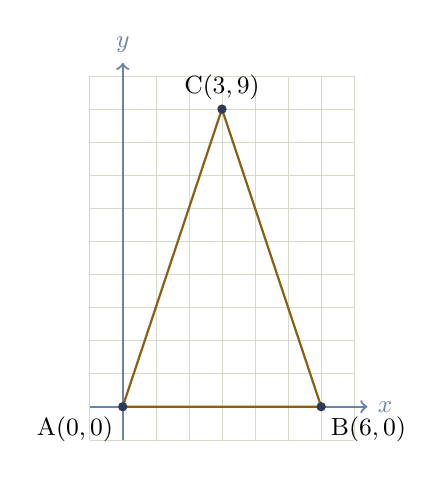
\begin{tikzpicture}[scale=0.42]
  \draw[step=1cm, linec, very thin] (-1,-1) grid (7,10);
  \draw[->, thick, indigosoft] (-1,0) -- (7.4,0) node[right, font=\small]{$x$};
  \draw[->, thick, indigosoft] (0,-1) -- (0,10.4) node[above, font=\small]{$y$};
  \draw[thick, goldstrong] (0,0) -- (6,0) -- (3,9) -- cycle;
  \filldraw[indigoc] (0,0) circle (3.5pt);
  \node[below left, font=\small] at (0,0) {A$(0,0)$};
  \filldraw[indigoc] (6,0) circle (3.5pt);
  \node[below right, font=\small] at (6,0) {B$(6,0)$};
  \filldraw[indigoc] (3,9) circle (3.5pt);
  \node[above, font=\small] at (3,9) {C$(3,9)$};
\end{tikzpicture}
\end{center}

\begin{enumerate}[leftmargin=1.4em, itemsep=2pt]
  \item 삼각형 ABC의 무게중심 G의 좌표를 구해 보자.
\end{enumerate}
\writespace{2}

\begin{enumerate}[leftmargin=1.4em, itemsep=2pt, start=2]
  \item 변 AB를 $2:1$로 내분하는 점 P, 변 BC를 $2:1$로 내분하는 점 Q, 변 CA를 $2:1$로 내분하는 점 R의 좌표를 각각 구해 보자.
\end{enumerate}
\writespace{4}

\begin{enumerate}[leftmargin=1.4em, itemsep=2pt, start=3]
  \item 삼각형 PQR의 무게중심을 구하고, 1번에서 구한 G와 비교해 보자. 무엇을 발견했는가?
\end{enumerate}
\writespace{3}
\end{sheetbox}

\section{탐구 \& 융합 --- 내분과 황금비}

\begin{sheetbox}
선분 AB 위의 점 P가
\[
\overline{AP} : \overline{PB} = \overline{AB} : \overline{AP}
\]
를 만족시킬 때, 점 P는 선분 AB를 \textbf{황금분할}한다고 하며, 이때의 비 $\overline{AB}:\overline{AP}$를 \textbf{황금비}라고 한다 (약 $1.618\,{:}\,1$). 파르테논 신전, 명함, 신용카드 등 여러 디자인에서 이 비율이 발견된다고 한다.

\vspace{8pt}
\textbf{직접 측정해 보기} --- 가지고 있는 명함, 신용카드, 교통카드, 스마트폰 화면 중 하나를 골라 가로·세로 길이를 재고, 그 비율이 황금비($1.618$)에 얼마나 가까운지 확인해 보자.

\begin{center}
\begin{tabular}{@{}p{3.2cm}p{2.6cm}p{2.6cm}p{3cm}@{}}
\toprule
측정한 물건 & 가로($a$) & 세로($b$) & $a\div b$ \\
\midrule
 & & & \\[10pt]
 & & & \\[10pt]
\bottomrule
\end{tabular}
\end{center}
\end{sheetbox}

\section{사고의 가시화 --- Connect · Extend · Challenge}

\noindent{\footnotesize\color{inksoft} 1$\sim$3차시 전체(선분의 내분)를 떠올리며 아래 세 칸을 채워 보자.}\\[6pt]
\begin{tabularx}{\linewidth}{@{}XXX@{}}
\textbf{\footnotesize\color{indigoc} Connect --- 무엇과 연결되나?} &
\textbf{\footnotesize\color{indigoc} Extend --- 어디까지 확장됐나?} &
\textbf{\footnotesize\color{indigoc} Challenge --- 아직 궁금한 것은?} \\[4pt]
\end{tabularx}
\noindent
\begin{minipage}[t]{0.32\linewidth}\writespace{3}\end{minipage}\hfill
\begin{minipage}[t]{0.32\linewidth}\writespace{3}\end{minipage}\hfill
\begin{minipage}[t]{0.32\linewidth}\writespace{3}\end{minipage}

\section{마무리 성찰}

\begin{sheetbox}
\begin{minipage}[t]{0.48\linewidth}
{\footnotesize\color{inksoft} `선분의 내분' 소단원을 마치며 한 문장으로}
\writespace{3}
\end{minipage}\hfill
\begin{minipage}[t]{0.48\linewidth}
{\footnotesize\color{inksoft} 감사 일기 / 유념 한 줄}
\writespace{3}
\end{minipage}
\end{sheetbox}

\end{document}
